\chapter{Dormand-Prince 5(4)}
In the following, we consider the initial value problem (IVP) on the form
\begin{align}
    \dot{x}(t) &= f(t,x(t),p), & x(t_0) = x_0,
\end{align}
where $x \in \probR ^{n_x}$ and $p \in \probR ^{n_p}$. 

\section{Description of Dormand-Prince 5(4)}
The Dorman-Prince 5(4) (DoPri54) method is to a large extend inspired by the classical Runge-Kutta, RK4, outlined in the previous chapter. They are both explicit Runge-Kutta methods, and as such are neither A- nor L-stable regarding the test equation. In practise, DoPri54 is one of the most used methods for solving IVPs on the form given above. In Matlab, it is the method used in the function \textit{ode45}. 

For typical Runge-Kutta methods, we can estimate the errors of the steps by means of step doubling. However, instead of using step doubling to estimate the errors, we can instead use an \textit{embedded} error estimate. Consider the butcher tableau given below

\begin{align}
    \begin{array}{c|cccc}
         c_1 & & & &   \\
         c_2 & a_{21} & & & \\
         \vdots & \vdots  & \vdots & & \\
         c_s & a_{s1} & a_{s2} & \cdots & \\ \hline 
         x & b_1 & b_2 & \cdots & b_s \\
         \hat{x} & \hat b_1 &  \hat b_2 & \cdots & \hat b_s \\ \hline
         e & d_1 & d_2 & \cdots & d_s
    \end{array}
\end{align}

as with RK4 we have 

\begin{align}
    T_i &= t+c_i \cdot h, \quad i = \{1,2,...,s\}\\
    X_i &= x_n + h \cdot \sum_{j=i}^{i-1} a_{ij} f(T_j, X_j), \quad i = \{1,2,...,s\}, \ and \\
    x_{n+1} &= x_n + h \cdot \sum_{i=1}^s b_i f(T_i,X_i).
\end{align}

Now we additionally have 

\begin{align}
    \hat x_{n+1} &= x_n + h \cdot \sum_{i=1}^s \hat b_i f(T_i,X_i) \\
    e_{n+1} &= x_{n+1} - \hat x_{n+1} = h \cdot \sum_{i=1}^s d_i f(T_i,X_i)
\end{align}
where $x_n=x(t_n)$, and $e_n = e(t_n)$. Now we will by design have an error estimate, $e(t)$. The accuracy of the estimate naturally depends on the specific tableau. The reason for using a method with an embedded error estimate is to avoid having to solve multiple steps. Computers are very good at solving linear algebra and as such it can give a computational advantage to use embedded errors estimates compared to step doubling. 

Dormand-Prince 5(4) is a 5th order, 7 stage Runge-Kutta method with embedded error estimation of 4th order. The specific butcher tableau is given by 

\begin{align}
        \begin{array}{c|ccccccc}
0	&0 &&&&&& \\
\frac{1}{5}	&\frac{1}{5} &&&&&& \\
\frac{3}{10}	&\frac{3}{40}	&\frac{9}{40} &&&&& \\
\frac{4}{5}	&\frac{44}{45}	&-\frac{56}{15}	&\frac{32}{9} &&&& \\
\frac{8}{9}	& \frac{19372}{6561}	&-\frac{25360}{2187}	& \frac{64448}{6561}	&-\frac{212}{729} &&& \\
1	&\frac{9017}{3168}	&-\frac{355}{33}	&\frac{46732}{5247}	&\frac{49}{176}	&-\frac{5103}{18656} && \\
1	&\frac{35}{384}	&0	&\frac{500}{1113}	&\frac{125}{192}	&-\frac{2187}{6784}	&\frac{11}{84}	& \\ \hline
x& \frac{35}{384}	&0	&\frac{500}{1113}	&\frac{125}{192}	&-\frac{2187}{6784}	&\frac{11}{84}	&0 \\
\hat{x}&\frac{5179}{57600}	&0	&\frac{7571}{16695}	&\frac{393}{640}	&-\frac{92097}{339200}	&\frac{187}{2100}	&\frac{1}{40} \\ \hline
e & \frac{71}{57600} &0 & -\frac{71}{16695} &\frac{71}{1920} &-\frac{17253}{339200} & \frac{22}{525} &-\frac{1}{40}
    \end{array}
\end{align}

We are now able to define how to select the best step size, $h$. We do so by the \textit{asymptotic step size controller}, this means that our step size is given by
\begin{align}
    h_{k+1} &= \left(\frac{\varepsilon}{r_{k+1}} \right )^{1/6} h_k.
\end{align}
Where $r_{k+1}$ is found by
\begin{align}
    r_{k+1} &= \max_{i \in \{1,...,n_x\}} \left \{ \frac{|e_{k+1}|_i}{ \max \{ |\text{abstol}|_i, \ |x_{k+1}|_i \cdot |\text{reltol}|_i \} } \right \}
\end{align}
where $|\text{abstol}|_i$ and $|\text{reltol}|_i$ are the absolute and relative tolerance of $(x_{k+1})_i$ respectively.

\section{Implementation of Dormand-Prince 5(4)}
Listing \ref{lst6:DoPri54} shows a Matlab implementation of a general explicit Runge-Kutta method with embedded error estimates. The specific parameters that correspond to DoPri54 are listed below the function. 

In the code we see that lines 2-12 initializes parameters, lines 15-17 determines if the an algorithm sould be run to estimate the best initial step size. Line 20 the main loop is initiated, $x_n$, $\hat x_n$, $e_n$ and $r_n$ are estimated. If $r_n \leq 1$ (line 35) we take one step, else we do not. Then the step size, $h$, is estimated (line 43), and if we did take a step, the new values are stored.

\begin{lstlisting}[language=Matlab,caption=Implementation of explicit Runge-Kutta solver with adaptive time step using embedded error estimates. Parameters corresponding to DoPri54 given at the end,label=lst6:DoPri54]
function [x,t,function_calls,hs] = explicitRungeKuttaEmbedded(f,param,h,t0,T,x0,A,b,bhat,c,Atol,Rtol,hmin,hmax,eps_tol,p,initial_step_algo)
    N = ceil((T-t0)/hmin);
    s = length(b);
    d = length(x0);
    t = zeros(1,N+1);
    hs = zeros(1,N+1);
    x = zeros(length(x0),N+1);
    k = zeros(d,s)';
    t(1) = t0;
    x(:,1) = x0;
    accept_step = false;
    function_calls = 0;
    
    
    if initial_step_algo % slide 4b, 9 whic is from p169 Hairer
        [h,function_calls] = initialStepSize(f,param,t0,x0);
    end
    
    i = 2;
    while t(i-1)<=T
        
       while(~accept_step)
           k = 0*k;
           for j = 1:s
               k(j,:) = f(t(i-1)+h*c(j),x(:,i-1)+sum(h*k.*A(j,:)',1)', param);
               function_calls = function_calls +1;
           end
           oneAhead = x(:,i-1)+sum(h*k.*b,1)';
           oneAheadhat = x(:,i-1)+sum(h*k.*bhat,1)';
           
           % Embedded error estimate
           e = abs(oneAhead-oneAheadhat);
           r = max(e./max(Atol,abs(oneAhead).*Rtol));
           
           if r<=1
               x(:,i) = oneAhead;
               hs(i-1) = h;
               t(i) = t(i-1)+h;
               accept_step = true;
           else
               accept_step = false;
           end
           h = h*max(hmin,min(hmax,(eps_tol/r)^(1/(1+p)))); % eq 4.13 in Harier
           
       end
       accept_step = false;
       i = i+1;
    end
    x = x(:,1:i-1)';
    t = t(1:i-1);
    hs = hs(1:i-2);
end

%% DoPri54 parameters
c = [0 1/5 3/10 4/5 8/9 1 1]';
A = [0 0 0 0 0 0 0 ;
     1/5 0 0 0 0 0 0
     3/40 9/40 0 0 0 0 0 ;
     44/45 -56/15 32/9 0 0 0 0 ;
     19372/6561 -25360/2187 64448/6561 -212/729 0 0 0;
     9017/3168 -355/33 46732/5247 49/176 -5103/18656 0 0;
     35/384 0 500/1113 125/192 -2187/6784 11/84 0];
b = [35/384 0 500/1113 125/192 -2187/6784 11/84 0]';
bhat = [5179/57600 0 7571/16695 393/640 -92097/339200 187/2100 1/40]';
p = 5;
\end{lstlisting}

\section{Test on the test equation}
As previously mentioned, \textit{stability}, i.e., how the methods converge, of numerical methods are an important characteristic of any numerical method. We have introduced the test equation in chapter 1, and we will use this to say something about the stability of numerical methods. It is important to remember that stability is seen in this exact context, i.e., how the method perform on the test equation with a given set of parameters. 

Again, we define the stability function, $R(\mu)$, by the relation

\begin{align}
    x(t+h) &= R(\mu) x(t).
\end{align}

Now, cf Ascher\cite{Ascher} (alternatively slide 8B), we know that for Runge Kutta methods we have

\begin{align}
    R(\mu) &= 1 + \mu b^T (I-\mu A)^{-1} e.
\end{align}

Then
\begin{align}
    e_{n+1} &= x_{n+1} - x(t_{n+1}) = \left [ R(\mu) - exp(\mu) \right] x_n.
\end{align}

The stability function now simplifies to 

\begin{align}
    R(\mu) &= 1 + \mu + \frac{\mu^2}{2} + \frac{\mu^3}{6} + \frac{\mu^4}{24} + \frac{\mu^5}{120} + \frac{\mu^6}{600}.
\end{align}

We remember that the stability region is given by

\begin{align}
    \mathcal{S} = \left \{ \mu \in \mathcal{C} \ | \ |R(\mu)| \leq 1 \right \}.
\end{align}

Figure \ref{fig6:dopri_stability} shows the stability region of the Dormand-Prince 5(4) method. As previously stated, the method is neither A- nor L-stable. 

\begin{figure}[H]
    \centering
    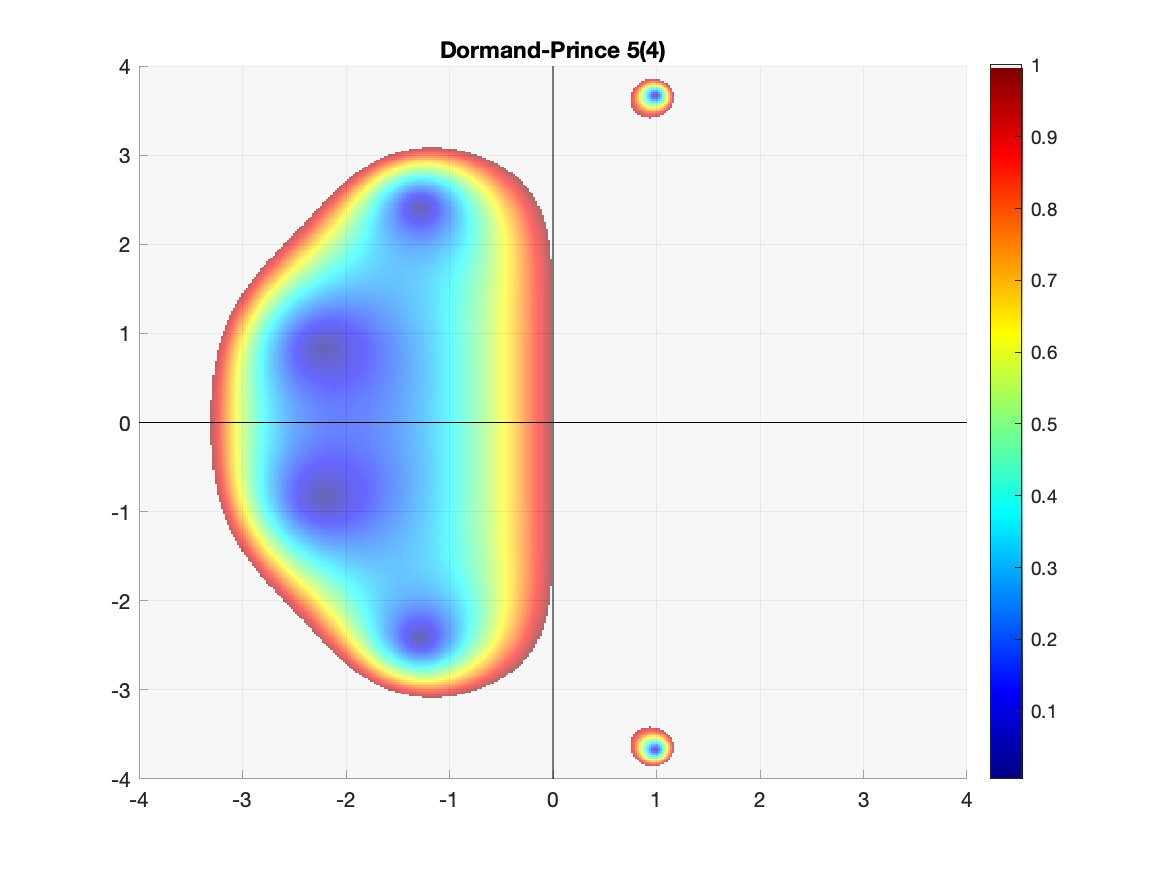
\includegraphics[width=10cm]{graphics/opg6/dopri-stability.png}
    \caption{Stability region of Dormand-Prince 5(4) method on test equation. The colored region is the stable region.}
    \label{fig6:dopri_stability}
\end{figure}


Regarding the order of the DoPri54, it is tedious to show a full proof of the order, as it required knowledge about \textit{rooted trees} and Hopf algebra. However, in Ascher\cite{Ascher} it is shown that DoPri54 has order 5, and the error estimate has order 4. 

Figure \ref{fig6:test_problem} shows the solution, local truncation error and global truncation error for the test problem with a fixed step size of $h=1$. Additionally, it also shows the analytical errors, i.e., the errors we expect DoPri54 to make with this step size. Notice how the dots are the discrete realizations of the analytical curves. 

\begin{figure}[H]
    \centering
    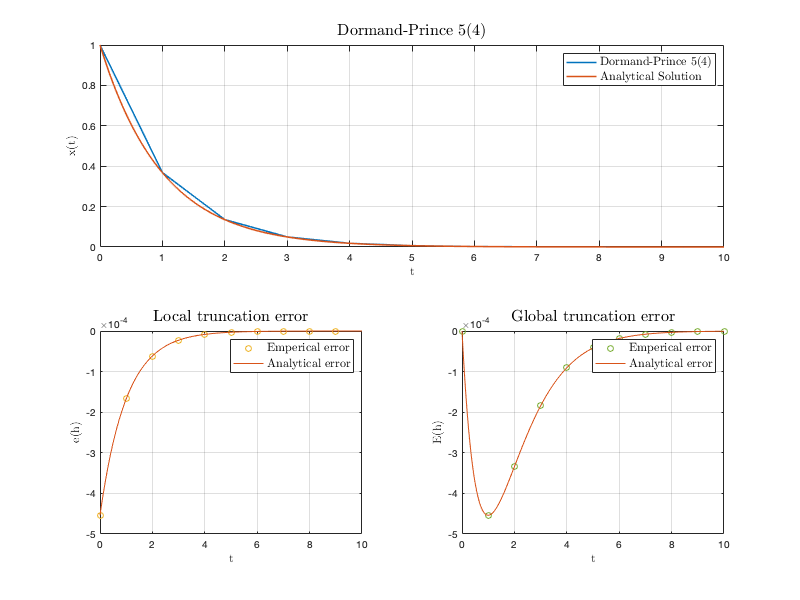
\includegraphics[width=10cm]{graphics/opg6/test_problem.png}
    \caption{Solution, local truncation error and global truncation error for the test problem}
    \label{fig6:test_problem}
\end{figure}



\section{Test on Van der Pol problem and comparison with Matlab ODE solvers}
Now that we have made an implementation of DoPri54 with adaptive step size we want to test it. To do so we look at the Van der Pol problem given by
\begin{align}
    \Ddot{x}(t) &= \mu (1-x(t)^2) \dot{x}(t) - x(t).
\end{align}
To solve the problem we must first re-write the problem as a system of first order differential equations. Luckily this is done easily and given by
\begin{align}
    \dot{x}_1(t) &= x_2(t) \\
    \dot{x}_2(t) &= \mu(1-x_1(t)^2) x_2(t) - x_1(t).
\end{align}

We will now test DoPri54 on the Van der Pol problem with $\mu = 3$ and $\mu = 20$. 

\subsection{Van der Pol, $\mu = 3$}
Figure \ref{fig6:adap_mu3} shows the numerical solution to the Van der Pol problem with $\mu = 3$ for DoPri54 with adaptive time steps and $AbsTol=RelTol \in \{10^{-2}, 10^{-4}, 10^{-6}\}$, ODE45 and ODE15s. Notice also that for $Tol = 10^{-2}$ we see some difference in the plots. It is simply because at the tolerance, DoPri54 take such large time steps, that we can see the straight lines by Matlab. This is especially visible in the "corner" of the solution curve.

\begin{figure}[H]
    \centering
    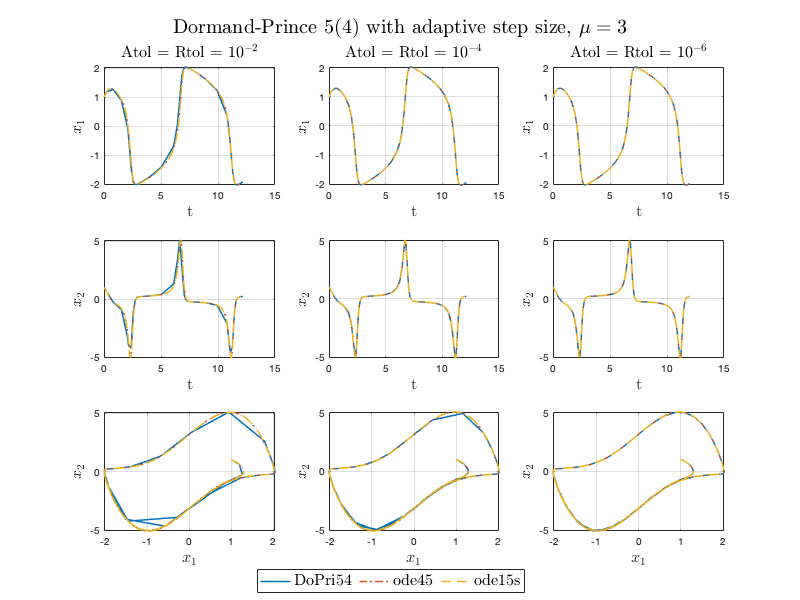
\includegraphics[width=\textwidth]{graphics/opg6/mu3_adap.png}
    \caption{Solution to Van der Pol with $\mu = 3$ using adaptive step sizes}
    \label{fig6:adap_mu3}
\end{figure}

Table \ref{tab6:mu3_adap} shows the CPU time and number of function evaluations when solving the Van der Pol problem with $\mu = 3$ using different tolerances and Matlab ODE solvers. Notice that with $Tol = 10^{-2}$ the DoPri54 is relatively fast (slower than ODE45 but faster than ODE15s). Generally, it is very hard to tell the solutions curves apart just by looking at them. Even for the lowest tolerance, we get quite good results. What is interesting is the CPU time usage and number of function evaluations used at the different tolerances. For both explicit- and implicit Euler, we saw that the CPU time and function evaluations increased dramatically when we required higher accuracy, now this increase is not as pronounced. This demonstrates the power of higher order methods quite well.

One of the reasons why ODE45 is able to outperform the DoPri45 with adaptive step size is because it has lower overhead. ODE45 uses the same algorithm as DoPri45, so we would expect the same asymptotic performance. Additionally, ODE45 might employ a different step size controller---this will obviously also affect the performance. 

\begin{table}[H]
    \centering
    \caption{CPU time and function evaluations of DoPri54 with adaptive time step and Matlab ODE solvers}
    \begin{tabular}{|c||c|c|c|c|c|c|} \hline
         \textbf{Method}    & $Tol = 10^{-2}$&   $Tol = 10^{-4}$ & $Tol = 10^{-6}$ & ODE45 & ODE15s     \\ \hline \hline 
         \textbf{Time}      & 0.0059  &  0.0376  &  0.0160 & 0.0046 & 0.0175   \\ \hline
         \textbf{Fun evals} & 373     &    681   &     1332 & 1069 & 926  \\ \hline
    \end{tabular}
    \label{tab6:mu3_adap}
\end{table}

Figure \ref{fig6:adap_mu3_h} shows the used step sizes for the different tolerances. The red crosses mark whenever the step size controller failed to set the step size correctly, i.e., whenever the estimated (using the embedded error estimate) error was larger than the allowed maximum. Notice that the behaviour of all three tolerances are quite similar. Also notice that the step sizes does not vary nearly as much for the individual tolerances as previously seen (for explicit- and implicit Euler). Additionally, if we look at the difference in step sizes for the different tolerances, we see that in order to decrease the tolerance by a factor $10^4$, we do not even need to decrease the step size by a factor $10^1$. This is the true power of higher order methods! And shows that the DoPri54 is indeed of order 5. 

\begin{figure}[H]
    \centering
    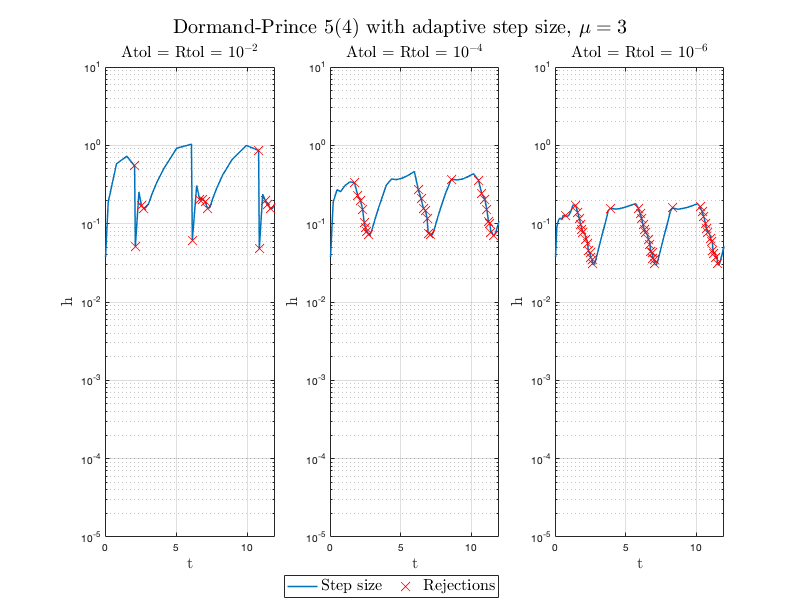
\includegraphics[width=\textwidth]{graphics/opg6/mu3_h.png}
    \caption{Step sizes when solving the Van der Pol with $\mu = 3$ at different tolerances}
    \label{fig6:adap_mu3_h}
\end{figure}

\subsection{Van der Pol, $\mu = 20$}
The Van der Pol problem with $\mu = 20$ is a more complicated problem. The dynamics of the problem is largely defined by the $\mu$ parameter. In particular, the problem becomes more stiff when $\mu$ is increased.

Figure \ref{fig6:adap_mu20} shows the numerical solution to the Van der Pol problem with $\mu = 20$ for DoPri54 with adaptive time steps and $AbsTol=RelTol \in \{10^{-2}, 10^{-4}, 10^{-6}\}$, ODE45 and ODE15s. Notice also that for $Tol = 10^{-2}$ the only difference visible is again due to the relatively large steps that the algorithm takes in the "non-stiff" area. Otherwise, all tolerances seem to follow the ODE45/ODE15s solutions very well.

\begin{figure}[H]
    \centering
    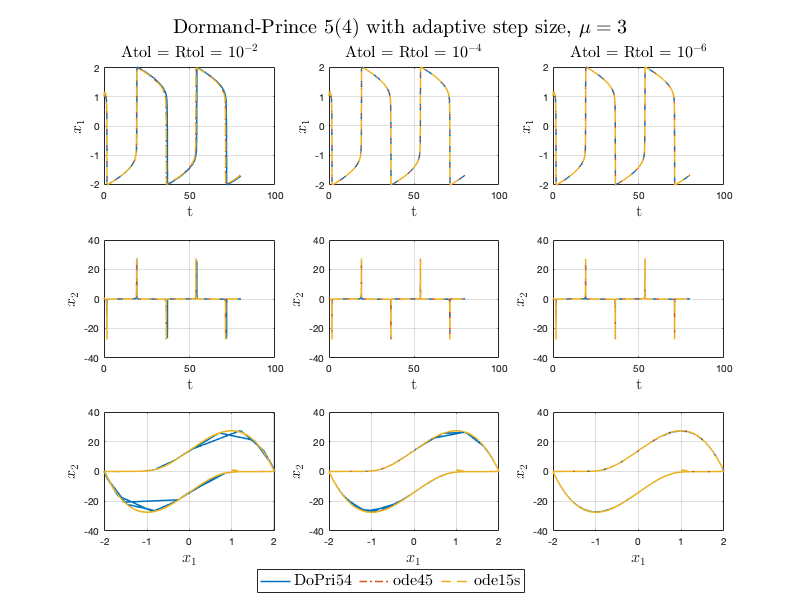
\includegraphics[width=\textwidth]{graphics/opg6/mu20_adap.png}
    \caption{Solution to Van der Pol with $\mu = 20$ using adaptive step sizes}
    \label{fig6:adap_mu20}
\end{figure}

Table \ref{tab6:mu20_adap} shows that CPU time and number of function evaluations when solving the Van der Pol problem with $\mu = 20$ using different tolerances and Matlab ODE solvers. Notice that with $Tol = 10^{-2}$ the DoPri54 is very similar in speed to ODE45 (and faster than ODE15s). Once again notice that 100 times the accuracy does not require 100 times the CPU time or 100 times the function calls. This is because DoPri54 is a 5th order method, i.e., the accuracy increase much faster than linear. Particular notice the relatively low difference in number of function calls between the tolerances.

\begin{table}[H]
    \centering
    \caption{CPU time and function evaluations of DoPri54 with adaptive time step and Matlab ODE solvers}
    \begin{tabular}{|c||c|c|c|c|c|c|} \hline
         \textbf{Method}    & $Tol = 10^{-2}$&   $Tol = 10^{-4}$ & $Tol = 10^{-6}$ & ODE45 & ODE15s     \\ \hline \hline 
         \textbf{Time}      & 0.0344 &   0.1419  &  0.2723 & 0.0386 & 0.0612   \\ \hline
         \textbf{Fun evals} &  6708    &    7422   &     9522 & 8461 & 2944  \\ \hline
    \end{tabular}
    \label{tab6:mu20_adap}
\end{table}

Figure \ref{fig6:adap_mu20_h} shows the used step sizes for the different tolerances. The red crosses mark whenever the step size controller failed to set the step size correctly, i.e., whenever the estimated error was larger than the allowed maximum. Notice that the behaviour of all three tolerances are not nearly as similar as previously seen. This time especially the most accurate tolerance struggles to determine the correct step sizes. This is mainly because the method generally takes very large steps (being a 5th order method), hence the change in step sizes can be very big in stiff areas. Also notice that the step sizes does not vary nearly as much for the individual tolerances as previously seen (for explicit- and implicit Euler). 

Finally, notice that the estimated step sizes are quite often rejected, i.e., the step size controller underestimated the need for more accuracy. Judging by the number of rejection for this fairly stiff problem, it might be worthwhile to consider other controller, e.g. a PID controller instead of the asymptotic step size controller we are currently using. 

\begin{figure}[H]
    \centering
    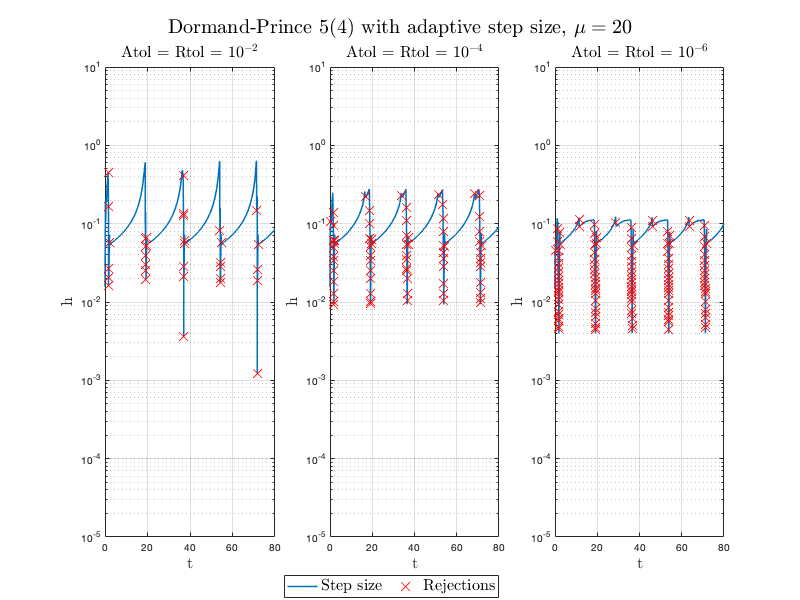
\includegraphics[width=\textwidth]{graphics/opg6/mu20_h.png}
    \caption{Step sizes when solving the Van der Pol with $\mu = 20$ at different tolerances}
    \label{fig6:adap_mu20_h}
\end{figure}


 
\section{Test on CSTR problem and comparison with Matlab ODE solvers}
To furhter test the DoPri54, we will also perform test on the adiabatic continuous stirred tank reactor (CSTR). The process is described in depth in \cite{cstr}, it is essentially a exothermic chemical reaction happening in two connected tanks. We will focus on the temperature of the tanks, and not look to much into the concentration of active compounds. 

The temperature of the CSTR problem is generally modelled by a system of three ODEs (where one is temperature), we will refer to this as the 3D system. However, as shown in the article, the dynamics of the temperature can be approximated by a single ODE, i.e., a 1D system. We will perform analysis of both the 1D and the 3D system.

The 1D CSTR system is given by

\begin{align}
    \dot T &=  \frac{F}{V} (T_{in} − T)+R_T (C_A(T),C_B(T),T)
\end{align}

and the 3D is given by

\begin{align}
\dot{C}_{A} &=\frac{F}{V}\left(C_{A, i n}-C_{A}\right)+R_{A}\left(C_{A}, C_{B}, T\right) \\
\dot{C}_{B} &=\frac{F}{V}\left(C_{B, i n}-C_{B}\right)+R_{B}\left(C_{A}, C_{B}, T\right) \\
\dot{T} &=\frac{F}{V}\left(T_{i n}-T\right)+R_{T}\left(C_{A}, C_{B}, T\right)
\end{align}

where all are constants. There is a small caveat---we will adjust the value of $F$ every 2 minutes. Figure \ref{fig6:f-val} shows the values of $F$ used in the CTSR problems. Notice we assume the value is modulated in 2min intervals. 

\begin{figure}[H]
    \centering
    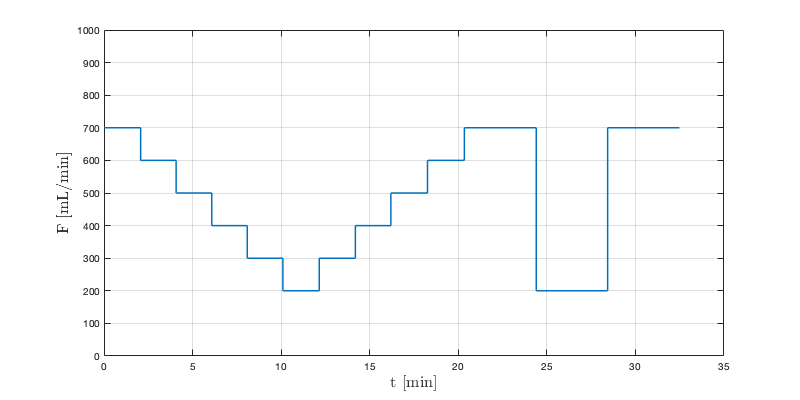
\includegraphics[width=\textwidth]{graphics/opg6/f-val.png}
    \caption{Value of $F$ as a function of time}
    \label{fig6:f-val}
\end{figure}

\subsection{1D}
We are now able to solve the IVP using the $F$ given above and constant parameters as given in \cite{cstr}. Figure \ref{fig6:1d_sol} shows the solution to the 1D CSTR using $AbsTol=RelTol \in \{10^{-2}, 10^{-4}, 10^{-6}\}$, together with solutions using ODE45 and ODE15s. For $Tol=10^{-2}$ we see some deviation from DoPri54 to ODE45/ODE15s, especially in areas where there is a fairly abrupt change in dynamics, i.e., areas that are stiff. For the tolerances $Tol \in \{10^{-4}, 10^{-6}\}$ there is no visible difference between the ODE45/ODE15s and DoPri54.

\begin{figure}[H]
    \centering
    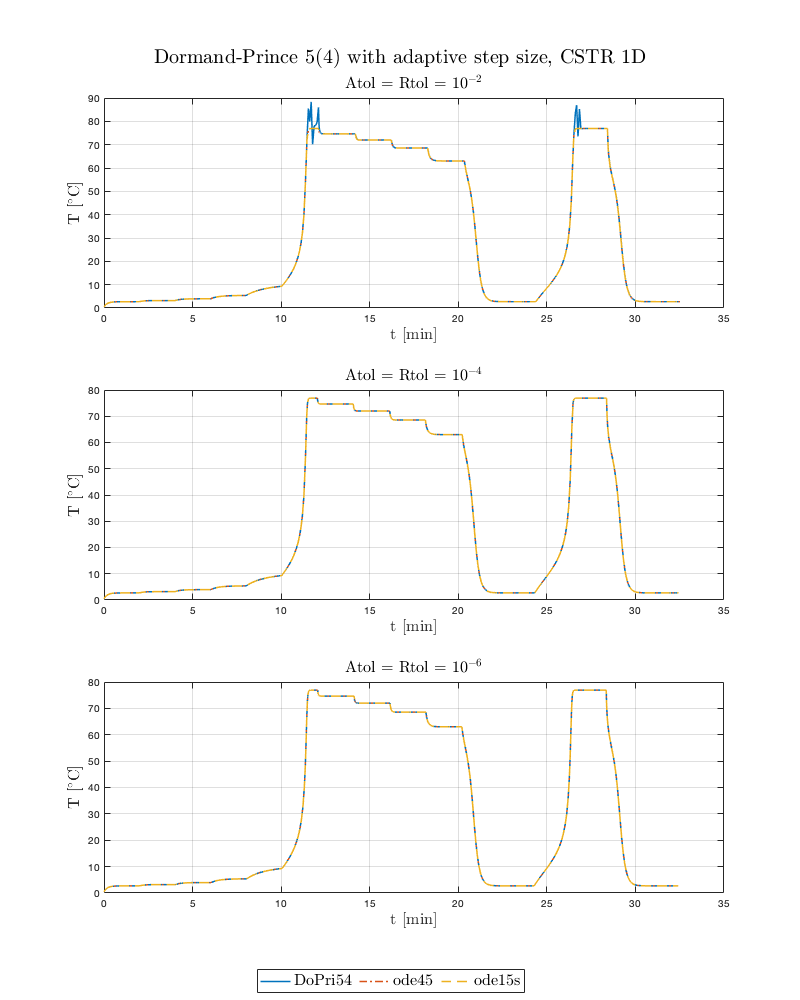
\includegraphics[width=\textwidth]{graphics/opg6/cstr-1d.png}
    \caption{Solutions to 1D CSTR using adaptive time step DoPri54}
    \label{fig6:1d_sol}
\end{figure}

Table \ref{tab6:1d_cstr} shows the CPU time and number of function evaluations for DoPri54 with varying tolerances, ODE45 and ODE15s. Notice that all DoPri45 methods use very similar number of function calls, and in fact they almost use exactly the same time. Notice also that ODE45 and ODE15s outperform DoPri54 quite dramicially, especially considering that they use more function calls. The reason for this is quite simply because ODE45/ODE15s has less overhead, i.e., it is not as expensive to call the function. In this setup, where all functions are call several times, this overhead becomes quite important. 

\begin{table}[H]
    \centering
    \caption{CPU time and function evaluations of DoPri54 with adaptive time step and Matlab ODE solvers}
    \begin{tabular}{|c||c|c|c|c|c|c|} \hline
         \textbf{Method}    & $Tol = 10^{-2}$&   $Tol = 10^{-4}$ & $Tol = 10^{-6}$ & ODE45 & ODE15s     \\ \hline \hline 
         \textbf{Time}      & 0.6190 &   0.5789  &  0.5667 & 0.0413 & 0.0814   \\ \hline
         \textbf{Fun evals} &  2902  &   2986    &  3266   &   5886 & 4308  \\ \hline
    \end{tabular}
    \label{tab6:1d_cstr}
\end{table}

Figure \ref{fig6:1d_h} shows the step sizes when solving the 1D CSTR using DoPri54 with adaptive time steps for the different tolerances. Notice that for the most part, the step sizes for the 3 tolerances are almost the same. This is because the CSTR problem for the most part is quite smooth, i.e., it is easy for good solver to find good solutions. However, there are some areas where the problem changes dynamics quite rapidly. We see this as very sudden drops in step sizes. Notice the difference between the drop at the different tolerances. For the low tolerance the drops are much deeper than for the large tolerance. This is seen as the deviations as discussed above.

\begin{figure}[H]
    \centering
    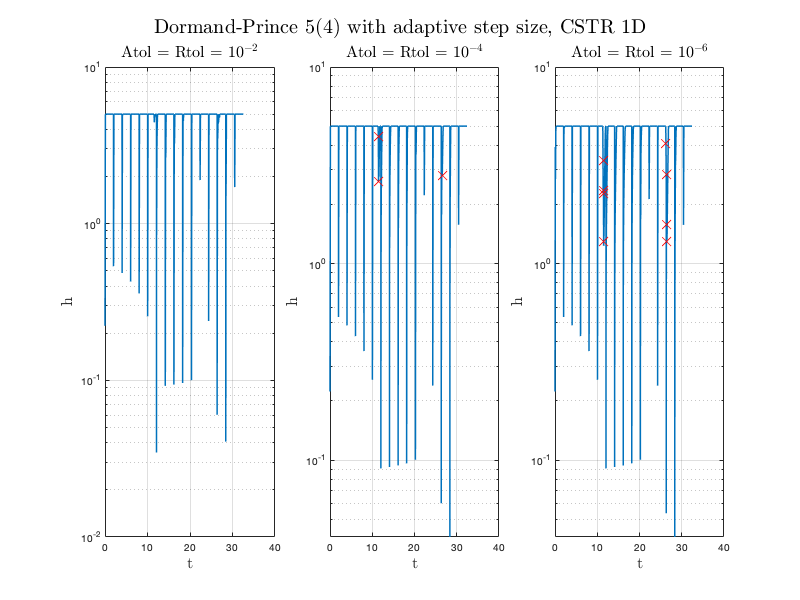
\includegraphics[width=\textwidth]{graphics/opg6/cstr_1d_h.png}
    \caption{Step sizes when solving the 1D CSTR using adaptive time step DoPri54}
    \label{fig6:1d_h}
\end{figure}

\subsection{3D}
Figure \ref{fig6:3d_sol} shows the solution to the 3D CSTR using $AbsTol=RelTol \in \{10^{-2}, 10^{-4}, 10^{-6}\}$, together with solutions using ODE45 and ODE15s. For $Tol=10^{-2}$ we see some deviation from DoPri54 to ODE45/ODE15s. This time the differences do not occur at the corner, but rather just after. For the tolerances $Tol \in \{10^{-4}, 10^{-6}\}$ there is no visible difference between the ODE45/ODE15s and DoPri54.

\begin{figure}[H]
    \centering
    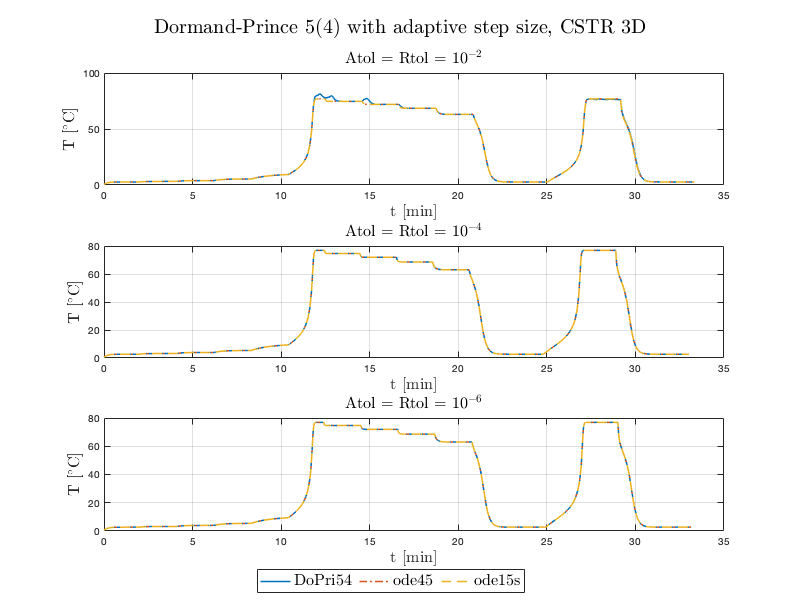
\includegraphics[width=\textwidth]{graphics/opg6/cstr-3d.png}
    \caption{Solutions to 3D CSTR using adaptive time step DoPri54}
    \label{fig6:3d_sol}
\end{figure}

Table \ref{tab6:3d_cstr} shows the CPU time and number of function evaluations for DoPri54 with varying tolerances, ODE45 and ODE15s. Notice that all DoPri45 methods use very similar number of function calls, and in fact they almost use exactly the same time. Notice also that ODE45 outperform DoPri54 quite dramatically, but this time ODE15s does not! For some reason our implementation of DoPri54 is faster for the 3D system than the 1D system. One possible reason for this is that that the 3D system is less stiff than the 1D system, and hence the optimal step size is easier obtained, and step sizes can be larger. Notice in particular the large difference in number of function calls between DoPri54 and ODE45/ODE15s. It seems that our implementation is able to take some really large steps.

\begin{table}[H]
    \centering
    \caption{CPU time and function evaluations of DoPri54 with adaptive time step and Matlab ODE solvers}
    \begin{tabular}{|c||c|c|c|c|c|c|} \hline
         \textbf{Method}    & $Tol = 10^{-2}$&   $Tol = 10^{-4}$ & $Tol = 10^{-6}$ & ODE45 & ODE15s     \\ \hline \hline 
         \textbf{Time}      & 0.2747 &   0.2420  &   0.2460 & 0.0899 & 0.6997   \\ \hline
         \textbf{Fun evals} &  1743     &   1477    &    2289   &  24828 & 15603  \\ \hline
    \end{tabular}
    \label{tab6:3d_cstr}
\end{table}

Figure \ref{fig6:3d_h} shows the step sizes when solving the 3D CSTR using DoPri54 with adaptive time steps for the different tolerances. Notice that for the most part, the step sizes for the 3 tolerances are almost the same. This is because the CSTR problem for the most part is quite smooth, i.e., it is easy for good solver to find good solutions. However, there are some areas where the problem changes dynamics quite rapidly. We see this as very sudden drops in step sizes. Notice the difference between the drop at the different tolerances. For the high tolerance the drops are much deeper than for the low tolerance. It seems that the asymptotic step size controller expects the most sudden change for the large tolerance. This might be the reason why the large tolerance is slower than the lower tolerances. Also notice that the step sizes are really large for some parts, with step sizes well above 10s! Finally, notice how much smoother this plot is compared to the 1D version. This really underlines that while the 1D version might be of lower dimension, that does not necessarily make it an easier problem. 

\begin{figure}[H]
    \centering
    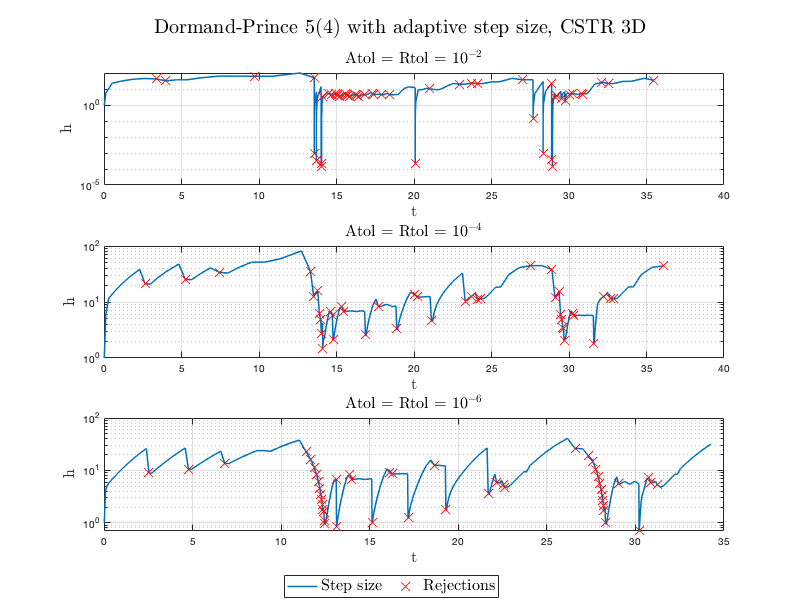
\includegraphics[width=\textwidth]{graphics/opg6/cstr_3d_h.png}
    \caption{Step sizes when solving the 3D CSTR using adaptive time step DoPri54}
    \label{fig6:3d_h}
\end{figure}






